% !TEX root = ../main.tex
\section{Числові характеристики випадкових величин}
\subsection{Математичне сподівання}

\begin{definition}
    \emph{Математичним сподіванням} випадкової величини називається
    інтеграл Стілтьєса
    \begin{equation}\label{eq:e_xi}
        E\xi = \int\limits_{-\infty}^{+\infty} x dF_\xi(x) = \begin{cases}
            \sum\limits_{k=1}^{n(\infty)} x_k P\left\{\xi = x_k\right\}, & \xi \text{ --- ДВВ} \\
            \int\limits_{-\infty}^{+\infty} x f_\xi(x)dx, & \xi \text{ --- НВВ}
        \end{cases}
    \end{equation}
\end{definition}
Інтеграл або ряд \eqref{eq:e_xi} має збігатися \emph{абсолютно}, інакше кажуть, що
випадкова величина не має математичного сподівання.
\begin{example}
    НВВ, розподілена за законом Коші з щільністю $f_\xi(x) = \frac{1}{\pi (1+x^2)}$
    не має математичного сподівання, бо інтеграл $\frac{1}{\pi}\int\limits_{-\infty}^{+\infty} \frac{x}{1+x^2}dx$ 
    розбіжний.
\end{example}
Математичне сподівання --- ймовірнісне середнє значення випадкової величини.
Фізична інтерпретація --- центр мас системи точок $\left\{x_1, x_2, ..., x_n,...\right\}$ з масами $\left\{p_1, p_2, ..., p_n, ...\right\}$ (ДВВ) або стрижня,
розподіл маси в якому задано функцією щільності (НВВ).

\noindent \textbf{Властивості математичного сподівання:}
\begin{enumerate}
    \item Математичне сподівання константи --- сама константа, оскільки
    її можна інтерпретувати як ДВВ, що приймає єдине значення з ймовірністю $1$.
    
    $c = const, E c = c$.
    \item $E \left(c\cdot\xi\right) = c\cdot E\xi$ --- властивість рядів та інтегралів.
    \item $E\left( \xi_1 + \xi_2\right) = E\xi_1 + E\xi_2$.
    \begin{proof}[Доведення для ДВВ]
        $P\left\{\xi_1 = x_k\right\} = p_k$, $P\left\{\xi_2 = y_j\right\} = p_j$, $P\left\{\xi_1 + \xi_2 = x_k + y_j\right\} = p_{kj}$.
        $E\left( \xi_1 + \xi_2\right) = \sum\limits_k \sum\limits_j (x_k+y_j) p_{kj} =
        \sum\limits_k x_k \sum\limits_j p_{kj} + \sum\limits_j y_j \sum\limits_k p_{kj} = \sum\limits_k x_k p_k + \sum\limits_j y_j p_j = E\xi_1 + E\xi_2$.
    \end{proof}
\suspend{enumerate}
\begin{definition}
    Дві випадкові величини $\xi_1$ та $\xi_2$, задані на одному ймовірнісному просторі, називаються \emph{незалежними}, якщо
    $\forall x, y$ події $A=\left\{\omega : \; \xi_1(\omega) < x\right\}$ та
    $B=\left\{\omega : \; \xi_2(\omega) < y\right\}$ є незалежними.
    В цьому випадку $P\left\{\xi_1 < x, \xi_2 < y\right\} = P(A \cap B) = P(A)\cdot P(B) = F_{\xi_1}(x)\cdot F_{\xi_2}(y)$.
\end{definition}
\resume{enumerate}
    \item Якщо $\xi_1$ та $\xi_2$ незалежні, то $E\xi_1\xi_2 = E\xi_1 \cdot E\xi_2$.
    \begin{proof}[Доведення для ДВВ]
        Позначимо $p_{kj} = P\left\{\xi_1 = x_k, \xi_2 = y_j\right\}$.
        $E\xi_1\xi_2 = \sum\limits_k \sum\limits_j x_k y_j p_{kj} = \sum\limits_k \sum\limits_j x_k y_j p_k p_j = \left( \sum\limits_k x_k p_k\right)\cdot \left( \sum\limits_j y_j p_j\right) = E\xi_1 \cdot E\xi_2$.
    \end{proof}
    Властивості 3 та 4 для НВВ буде доведено в темі <<Функції випадкових аргументів>>.
\end{enumerate}

\begin{example}
    \begin{enumerate}
        \item Обчислити математичне сподівання двох ДВВ:
        
        \begin{tabular}{c c}
            \begin{tabular}{|c|c|c|}
                \hline
                $\xi_1$ & $-1$ & $1$ \\ 
                \hline
                $p$ & $1/2$ & $1/2$ \\
                \hline
            \end{tabular} &
            \begin{tabular}{|c|c|c|}
                \hline
                $\xi_2$ & $-100$ & $100$ \\ 
                \hline
                $p$ & $1/2$ & $1/2$ \\
                \hline
            \end{tabular}
        \end{tabular}
        $E\xi_1 = -1\cdot \frac{1}{2} + 1\cdot \frac{1}{2} = 0, E\xi_2 = -100\cdot \frac{1}{2} + 100\cdot \frac{1}{2} = 0$.
        
        Цей приклад показує, що попри однакове значення математичного сподівання, можливі значення цих ДВВ знаходяться на різній відстані від нього.
        \item Обчислити математичне сподівання НВВ, розподіленої за законом Сімпсона.

        \begin{tabular}{c c}
            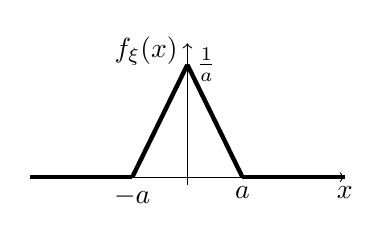
\begin{tikzpicture}[baseline={(current bounding box.center)}, yscale=1]
                \pgfmathsetmacro{\a}{0.7}
                \draw [->] (-2, 0) -- (2, 0);
                \draw [->] (0, -0.1) -- (0, 1.7);
                \draw [ultra thick] (-2, 0) -- (-\a, 0);
                \draw [ultra thick] (\a, 0) -- (2, 0);
                \draw [ultra thick] (-\a, 0) -- (0, 1/\a);
                \draw [ultra thick] (\a, 0) -- (0, 1/\a);
                \node [below] at (2, 0) {$x$};
                \node [left] at (0, 1.6) {$f_\xi(x)$};
                \node [below] at (\a, 0) {$a$};
                \node [below] at (-\a, 0) {$-a$};
                \node [right] at (0, 1/\a) {$\frac{1}{a}$};
            \end{tikzpicture} &
            $f_\xi(x) = \begin{cases}
                \frac{1}{a} \left(1 - \frac{|x|}{a}\right), & |x| \leq a \\
                0, & |x| > a
            \end{cases} (a>0)$
        \end{tabular}
        
        $E\xi = \int\limits_{-\infty}^{+\infty} x f_\xi(x)dx = \int\limits_{-a}^a \frac{x}{a}\left(1 - \frac{|x|}{a}\right)dx = 0$, 
        оскільки інтегрується непарна функція по симетричному проміжку.
    \end{enumerate}
\end{example}

\subsection{Дисперсія}
\begin{definition}
    \emph{Дисперсією} випадкової величини називається 
    \begin{equation}\label{eq:d_xi}
        D\xi = E\left(\xi-E\xi\right)^2 = \int\limits_{-\infty}^{+\infty} \left(x-E\xi\right)^2 dF_\xi(x) = \begin{cases}
            \sum\limits_{k=1}^{n(\infty)} \left(x_k-E\xi\right)^2 P\left\{\xi = x_k\right\}, & \xi \text{ --- ДВВ} \\
            \int\limits_{-\infty}^{+\infty} \left(x-E\xi\right)^2 f_\xi(x)dx, & \xi \text{ --- НВВ}
        \end{cases}
    \end{equation}
\end{definition}
Дисперсія --- характеристика розсіювання випадкової величини навколо свого математичного сподівання.
Фізична інтерпретація --- момент інерції маси системи точок або стрижня (як і у випадку інтерпретації математичного сподівання)
відносно свого центру мас.

\begin{example}
    \begin{enumerate}
        \item Обчислити дисперсії двох ДВВ:
        
        \begin{tabular}{c c}
            \begin{tabular}{|c|c|c|}
                \hline
                $\xi_1$ & $-1$ & $1$ \\ 
                \hline
                $p$ & $1/2$ & $1/2$ \\
                \hline
            \end{tabular} &
            \begin{tabular}{|c|c|c|}
                \hline
                $\xi_2$ & $-100$ & $100$ \\ 
                \hline
                $p$ & $1/2$ & $1/2$ \\
                \hline
            \end{tabular}
        \end{tabular}
        
        $D\xi_1 = (-1)^2\cdot \frac{1}{2} + 1^2\cdot \frac{1}{2} = 1, D\xi_2 = (-100)^2\cdot \frac{1}{2} + 100^2\cdot \frac{1}{2} = 10000$.
        \item Обчислити дисперсію НВВ, розподіленої за законом Сімпсона.
        
        Відповідна щільність розподілу має вигляд $f_\xi(x) = \begin{cases}
            \frac{1}{a} \left(1 - \frac{|x|}{a}\right), & |x| \leq a \\
            0, & |x| > a
        \end{cases}$.
        Математичне сподівання вже було обчислено, воно рівне 0. Тому $D\xi = \int\limits_{-\infty}^{+\infty} \left(x-E\xi\right)^2 f_\xi(x)dx =
        \int\limits_{-a}^a \frac{x^2}{a}\left(1 - \frac{|x|}{a}\right)dx = \frac{2}{a}\int\limits_0^a {x^2}\left(1 - \frac{x}{a}\right)dx =
        \frac{2}{a}\cdot \left( \frac{x^3}{3} - \frac{x^4}{4a}\right)\Bigr\vert_0^a = \frac{2}{a} \cdot \left( \frac{a^3}{3} - \frac{a^3}{4}\right) = \frac{a^2}{6}$.
    \end{enumerate}
\end{example}

\noindent \textbf{Властивості дисперсії:}
\begin{enumerate}
    \item $D\xi \geq 0$, $\sqrt{D\xi} = \sigma_\xi$ --- \emph{середньоквадратичне (стандартне) відхилення}.
    \item $D\xi = 0 \Leftrightarrow \xi = const$, бо $D c = E(c - Ec)^2 = 0$.
    \item Для обчислення дисперсії більш зручною є наступна формула:

    $D\xi = E(\xi^2 - 2\xi E\xi +(E\xi)^2) = E\xi^2 - 2(E\xi)^2 + (E\xi)^2 = E\xi^2 - (E\xi)^2$. 
    \item $D(c\cdot \xi) = c^2\cdot D\xi$, оскільки $D(c\cdot \xi) = E\left(c\cdot\xi-E(c\cdot\xi\right))^2 = E\left(c\cdot\xi - c\cdot E\xi\right)^2 = c^2 \cdot E\left(\xi-E\xi\right)^2 = c^2 \cdot D\xi$.
\suspend{enumerate}
\begin{definition}
    \emph{Центрованою} випадковою величиною, що відповідає випадковій величині $\xi$, називається 
    випадкова величина $\mathring{\xi} = \xi - E\xi$. Для неї $E\mathring{\xi} = 0$ та 
    $E\mathring{\xi^2} = D\xi$.
\end{definition}
\resume{enumerate}
    \item Якщо випадкові величини $\xi_1$ та $\xi_2$ --- незалежні, то
    $D\left(\xi_1 + \xi_2\right) = D\xi_1 + D\xi_2$.
    \begin{proof}
        $D\left(\xi_1 + \xi_2\right) = E((\xi_1 + \xi_2) - E(\xi_1 + \xi_2))^2 = E(\mathring{\xi}_1 + \mathring{\xi}_2)^2 =
        E\mathring{\xi}_1^2 + 2E\mathring{\xi}_1\mathring{\xi}_2 + E\mathring{\xi}_2^2 = 
        E\mathring{\xi}_1^2 + 2E\mathring{\xi}_1 E\mathring{\xi}_2 + E\mathring{\xi}_2^2 =
        E\mathring{\xi}_1^2 + E\mathring{\xi}_2^2 = D\xi_1 + D\xi_2$.
    \end{proof}
\end{enumerate}

\subsection{Моменти випадкової величини}
\begin{definition}
    \emph{Початковим моментом k-того порядку} ($k \in \mathbb{N}$) ВВ $\xi$ називається
    \begin{equation}\label{eq:e_alpha_k}
        \alpha_k = E\xi^k = \int\limits_{-\infty}^{+\infty} x^k dF_\xi(x) = \begin{cases}
            \sum\limits_{m=1}^{n(\infty)} x_m^k P\left\{\xi = x_m\right\}, & \xi \text{ --- ДВВ} \\
            \int\limits_{-\infty}^{+\infty} x^k f_\xi(x)dx, & \xi \text{ --- НВВ}
        \end{cases}
    \end{equation}
\end{definition}
\begin{definition}
    \emph{Центральним моментом k-того порядку} ($k \in \mathbb{N}$) ВВ $\xi$ називається
    \begin{equation}\label{eq:d_beta_k}
        \beta_k = E\mathring{\xi}^k = E\left(\xi-E\xi\right)^k = \int\limits_{-\infty}^{+\infty} \left(x-E\xi\right)^k dF_\xi(x) = \begin{cases}
            \sum\limits_{m=1}^{n(\infty)} \left(x_m-E\xi\right)^k P\left\{\xi = x_m\right\}, & \xi \text{ --- ДВВ} \\
            \int\limits_{-\infty}^{+\infty} \left(x-E\xi\right)^k f_\xi(x)dx, & \xi \text{ --- НВВ}
        \end{cases}
    \end{equation}
\end{definition}

\noindent \textbf{Зв'язок між центральними та початковими моментами}

$\beta_k = E\left(\xi-E\xi\right)^k = E\left( \sum\limits_{j=0}^k C_k^j \xi^j (-1)^{k-j} (E\xi)^{k-j}\right) =
\sum\limits_{j=0}^k (-1)^{k-j} C_k^j E\xi^j (E\xi)^{k-j}$.

\noindent Отже, $\beta_k = \sum\limits_{j=0}^k (-1)^{k-j} C_k^j \alpha_j (\alpha_1)^{k-j}$.
Частковим випадком цієї формули є формула для дисперсії: $D\xi = \beta_2 = \alpha_2 - \alpha_1^2 = E\xi^2 - (E\xi)^2$.
\begin{exercise}
    Виразити через початкові моменти $\beta_3$ та $\beta_4$.
\end{exercise}
Розглядаються також абсолютні початкові моменти $E\vert \xi \vert ^k$, абсолютні центральні моменти $E\vert \xi - E\xi \vert ^k$
та факторіальні моменти $\gamma_k = E\left( \xi (\xi - 1) ... (\xi - k + 1)\right)$.


\subsection{Мода та медіана випадкової величини}
\begin{definition}
    \emph{Модою} ${Mo}\xi$ називається абсциса точки максимуму щільності 
    розподілу у випадку НВВ та значення, ймовірність 
    появи якого є найбільшим у випадку ДВВ.

    \emph{Унімодальний закон} --- такий, що має лише одну моду. 
    \emph{Полімодальний закон} --- такий, що має декілька мод.
    \emph{Антимодальний закон} --- такий, що не має моди. Приклад --- закон арксинуса, щільність якого має лише точку мінімуму.
\end{definition}
\begin{definition}
    Точка $x_0$ називається \emph{медіаною} $Me\xi$, якщо 
    $P\left\{\xi < x_0\right\} = P\left\{\xi \geq x_0\right\} 
    = \frac{1}{2} \Leftrightarrow F_\xi(x_0) = \frac{1}{2}$.
    Медіана є окремим випадком \emph{квантиля}.
\end{definition}
\begin{definition}
    Точка $x_0$ називається \emph{квантилем q-го порядку} якщо $F_\xi(x_0) = q$.
\end{definition}
\begin{example}
    Знайти моду та медіану НВВ, розподіленої за законом Релея.
    
    \begin{tabular}{c c}
        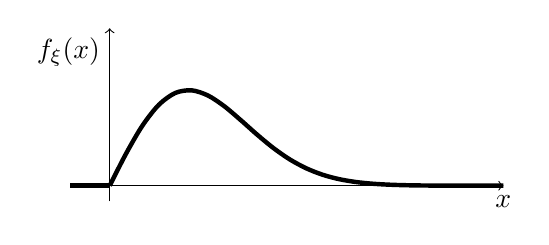
\begin{tikzpicture}[baseline={(current bounding box.center)}, yscale=2]
            \pgfmathsetmacro{\s}{1}
            \draw [->] (-0.5, 0) -- (5, 0);
            \draw [->] (0, -0.1) -- (0, 1);
            \node [below] at (5, 0) {$x$};
            \node [below left] at (0, 1) {$f_\xi(x)$};
            \draw [domain=0:5, smooth, variable = \x, ultra thick] plot ({\x}, {((\x/(\s^2)) * exp(-(\x)^2/(2*\s^2))});
            \draw [ultra thick] (-0.5, 0) -- (0, 0);
        \end{tikzpicture} &
        $f_\xi(x) = \begin{cases}
            \frac{x}{\sigma^2} e^{-\frac{x^2}{2\sigma^2}}, & x \geq 0 \\
            0, & x < 0
        \end{cases} (\sigma > 0)$ 
    \end{tabular}

    Для визначення моди знайдемо максимум $f_\xi(x)$ при $x\geq 0$.
    $f'_\xi(x) = \frac{\sigma^2 - x^2}{\sigma^4} e^{-\frac{x^2}{2\sigma^2}} = 0$ при $x=\sigma$.
    $f''_\xi(x) = \left( -\frac{3x}{\sigma^4} + \frac{x^3}{\sigma^6}\right) e^{-\frac{x^2}{2\sigma^2}}$,
    $f''_\xi(\sigma) = -\frac{2}{\sigma^3} e^{-\frac{1}{2}} < 0$. Отже, в точці $x=\sigma$ дійсно максимум $f_\xi(x)$, тому $Mo\xi = \sigma$.

    Медіану знайдемо з рівності $P\left\{\xi < x_0\right\} = 0.5$. $P\left\{\xi < x_0\right\} = \int\limits_{-\infty}^{x_0}f_\xi(x)dx = 
    \int\limits_0^{x_0} \frac{x}{\sigma^2} e^{-\frac{x^2}{2\sigma^2}} dx = 1 - e^{-\frac{x_0^2}{2\sigma^2}}$.
    З рівняння $1 - e^{-\frac{x_0^2}{2\sigma^2}} = 0.5$ знаходимо $x_0 = \sigma \sqrt{2\ln{2}}$.
\end{example}

\subsection{Асиметрія та ексцес випадкової величини}
\begin{definition}
    \emph{Асиметрією} випадкової величини $As\xi$ називається безрозмірна 
    числова характеристика, що дорівнює $\frac{\beta_3}{\sigma_\xi^3} = 
    \frac{E(\xi - E\xi)^3}{(D\xi)^{3/2}}$. 
    Ця характеристика показує порушення чи наявність симетрії кривої розподілу відносно математичного сподівання.
\end{definition}
\begin{tabular}{c c c}
    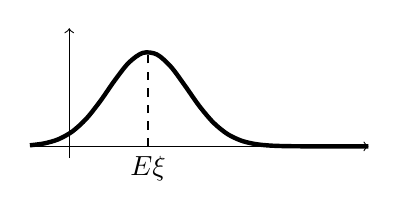
\begin{tikzpicture}[yscale = 1.5]
        \draw [->] (-0.5, 0) -- (3.8, 0);
        \draw [->] (0, -0.1) -- (0, 1);
        \draw [domain=-0.5:3.8, smooth, variable = \x, ultra thick] plot ({\x}, {0.797884560803 * exp(-2*(\x-1)^2)});
        \draw [dashed] (1, 0) -- (1, 0.797884560803);
        \node [below] at (1, 0) {$E\xi$};
    \end{tikzpicture} &
    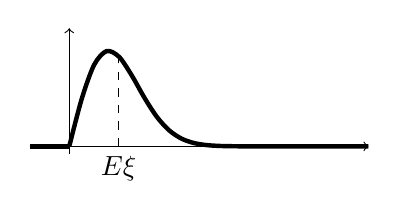
\begin{tikzpicture}
        \pgfmathsetmacro{\s}{0.5}
        \draw [domain=0:3.8, smooth, variable = \x, ultra thick] plot ({\x}, {((\x/(\s^2)) * exp(-(\x)^2/(2*\s^2))});
        \draw [ultra thick] (-0.5, 0) -- (0, 0);
        \draw [->] (-0.5, 0) -- (3.8, 0);
        \draw [->] (0, -0.1) -- (0, 1.5);
        \draw [dashed] (0.6267, 0) -- (0.6267, 1.143);
        \node [below] at (0.6267, 0) {$E\xi$};
    \end{tikzpicture} &
    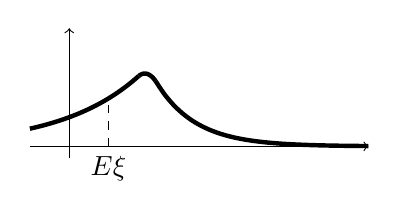
\begin{tikzpicture}[yscale = 1.5]
        \draw [->] (-0.5, 0) -- (3.8, 0);
        \draw [->] (0, -0.1) -- (0, 1);
        \draw [domain=-0.5:0.8846, smooth, variable = \x, ultra thick] plot ({\x}, {0.67*exp(\x-1)});
        \draw [domain=0.8846:1.0947, smooth, variable = \x, ultra thick] plot ({\x}, {0.67*(-5.1*(\x-0.96)^2 + 0.92)});
        \draw [domain=1.0947:3.8, smooth, variable = \x, ultra thick] plot ({\x}, {0.67*exp(-2*\x+2)});
        \draw [dashed] (0.4977, 0) -- (0.4977, 0.4053);
        \node [below] at (0.4977, 0) {$E\xi$};
    \end{tikzpicture} \\
    $As\xi = 0$ & $As\xi < 0$ & $As\xi > 0$ 
\end{tabular}
\begin{definition}
    \emph{Ексцесом} випадкової величини $Ex\xi$ називається безрозмірна 
    числова характеристика, що дорівнює $Ex\xi = \frac{\beta_4}{\sigma_\xi^4} - 3 = 
    \frac{E(\xi - E\xi)^4}{(D\xi)^{2}} - 3$.
    Ця характеристика показує, наскільки швидко крива розподілу 
    прямує до точки максимуму.
\end{definition}
\begin{center}
    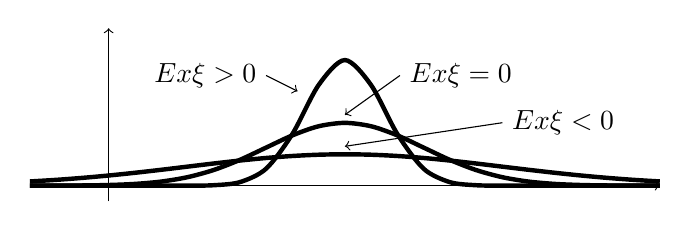
\begin{tikzpicture}[yscale = 2]
        \draw [->] (-1, 0) -- (7, 0);
        \draw [->] (0, -0.1) -- (0, 1);
        \draw [domain=-1:7, smooth, variable = \x, ultra thick] plot ({\x}, {0.398942280401 * exp(-(\x-3)^2/2)});
        \draw [domain=-1:7, smooth, variable = \x, ultra thick] plot ({\x}, {0.797884560803 * exp(-2*(\x-3)^2)});
        \draw [domain=-1:7, smooth, variable = \x, ultra thick] plot ({\x}, {0.199471140201 * exp(-(\x-3)^2/8)});
        \draw [->] (2, 0.7) -- (2.4, 0.6);
        \node [left] at (2, 0.7) {${Ex}\xi > 0$};
        \draw [->] (3.7, 0.7) -- (3, 0.45);
        \node [right] at (3.7, 0.7) {${Ex}\xi = 0$};
        \draw [->] (5, 0.4) -- (3, 0.25);
        \node [right] at (5, 0.4) {${Ex}\xi < 0$};
    \end{tikzpicture}
\end{center}

\subsection{Метод генератрис при вивченні ДВВ}
\begin{definition}
    Нехай $\xi$ --- ДВВ, що приймає цілі невід'ємні значення. 
    \emph{Генератрисою} цієї ДВВ називається функція комплексного аргументу
    \begin{equation}\label{eq:gen_func}
        \varphi_\xi(z) = \sum\limits_{k=0}^{\infty} P\left\{\xi = k\right\} z^k
    \end{equation}
\end{definition}
\noindent \textbf{Властивості генератриси:}
\begin{enumerate}
    \item Відповідний ряд рівномірно збігається принаймні в колі $|z|\leq 1$.
    \begin{proof}
        $\left| \sum\limits_{k=0}^{\infty} P\left\{\xi = k\right\} z^k \right| \leq \sum\limits_{k=0}^{\infty} P\left\{\xi = k\right\} = 1$.
    \end{proof}
    \item Генератриса --- аналітична функція в колі $|z|\leq 1$.
    \item За генератрисою можна відновити розподіл $\xi$:
    $P\left\{\xi = k\right\} = \frac{\varphi_\xi^{(k)}(0)}{k!}$.
    \item За допомогою генератриси можна знайти початкові та факторіальні моменти $\xi$.
    \begin{proof}
        За означенням факторіальний момент $\gamma_m = E\left( \xi (\xi - 1) ... (\xi - m + 1)\right)$.
        Для ДВВ, що розглядаються, він рівний $\sum\limits_{k=0}^{\infty} k(k-1)(k-2)...(k-m+1) P\left\{\xi = k\right\}$.
        З іншого боку, $\varphi'_\xi(z) = \sum\limits_{k=0}^{\infty} k P\left\{\xi = k\right\} z^{k-1}$,
        $\varphi''_\xi(z) = \sum\limits_{k=0}^{\infty} k(k-1) P\left\{\xi = k\right\} z^{k-2}$ і так далі,
        $\varphi^{(m)}_\xi(z) = \sum\limits_{k=0}^{\infty} k(k-1)(k-2)...(k-m+1) P\left\{\xi = k\right\} z^{k-m}$.
        Отже, $\gamma_m = \varphi^{(m)}_\xi(1)$.
        
        Тепер нескладно знайти, наприклад, математичне сподівання та дисперсію.
        Факторіальний та початковий моменти першого порядку збігаються, тому $E\xi = \varphi'_\xi(1)$.
        Дисперсію знайдемо за допомогою другого факторіального моменту: $\gamma_2 = E\left( \xi (\xi - 1)\right) = E\xi^2 - E\xi = \varphi''_\xi(1)$,
        звідки $E\xi^2 = \varphi''_\xi(1) + \varphi'_\xi(1)$. 
        Отже, $D\xi = E\xi^2 - (E\xi)^2 = \varphi''_\xi(1) + \varphi'_\xi(1) - \left( \varphi'_\xi(1)\right)^2$.
    \end{proof}
\end{enumerate}
\begin{exercise}
    Виразити через похідні генератриси центральні моменти 3-го та 4-го порядків.
\end{exercise}